\chapter{Introducción}
\label{cap:capitulo1}
\setcounter{page}{1}

\vspace{0.25cm}

\section{Contexto y motivación}
\label{sec:segundaseccion}

Los robots paralelos accionados por cables, también conocidos como Cable Driven Parallel Robots (CDPR), han despertado bastante interés en los últimos años tanto en el ámbito académico como en el ámbito industrial. Este tipo de robots basa su funcionamiento en el uso de cables que pueden ser recogidos o elongados por poleas con el objetivo de desplazar el efector final que une todos los cables a una posición específica, obteniendo como resultado una estructura ligera, escalable, y lo más importante de todo, capaz de realizar grandes volúmenes de trabajo en comparación con otros tipos de robots.

\vspace{0.25cm}

Durante los últimos seis años, los cuales he dedicado enteramente a mi formación en el Grado en Ingeniería de Robótica Software, y tras haber abordado diferentes campos de la robótica, he decidido decantarme por este tipo de robots como tema principal de mi TFG, ya que combina conceptos de modelado matemático y cinemático, el uso de un lenguaje de programación de alto nivel como lo es Python, y una de las arquitecturas software por excelencia utilizadas en el mundo de la robótica: ROS 2. Este Trabajo de Fin de Grado tiene como objetivo principal la profundización en el diseño y el desarrollo de un CDPR de dos grados de libertad desde un punto de vista práctico y orientado al software.

\begin{figure} [h!]
    \begin{center}
        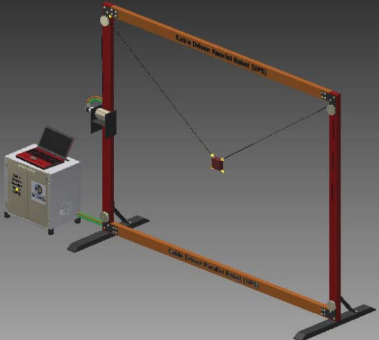
\includegraphics[width=0.5\textwidth]{figs/cdpr_model.png}
    \end{center}
    \caption{Ejemplo visual de un CDPR de dos grados de libertad}
\end{figure}\

\newpage

Y por último, es importante mencionar que la principal motivación que me ha llevado a elegir este tipo de robots como tema principal de mi TFG es que el comportamiento global del sistema viene determinado principalmente por la correcta formulación del modelo cinemático, además de todo lo que respecta a la implementación software.

\section{Planteamiento del problema}
\label{sec:segundaseccion}

El problema principal que se aborda en este TFG es el control de la posición de un efector final suspendido mediante dos cables ubicados en una estructura fija, en este caso una pizarra móvil con ruedas, a través de poleas, donde el sistema debe ser capaz de desplazar el efector final hacia una o varias posiciones específicas, siendo capaz de definir trayectorias en caso de que el efector final pase por más de una posición, todo ello dentro de una región bidimensional cuadrada cuya área cuadrada viene definida por la distancia que separa ambas poleas.

\vspace{0.25cm}

Sabiendo esto, es necesario establecer una relación entre la región por la que se mueve el efector final y las variables físicas del sistema, como por ejemplo las longitudes de los cables y el ángulo que debe rotar cada polea para desplazar el efector final a una posición específica. Esta relación debe ser lo suficientemente robusta de forma que pueda implementarse en un entorno real, y lo suficientemente flexible como para poder integrarla en software robótico.

\newpage

En este TFG me he centrado principalmente en desarrollar todo el software necesario para resolver este problema, dejando la implementación del sistema real como una fase posterior, actualmente en proceso de definición y que abordaré en conjunto con mi tutor de TFG, \href{https://github.com/juanscelyg}{Juan Sebastián Cely Gutiérrez}.

\section{Objetivos}
\label{sec:segundaseccion}

El objetivo principal de este TFG consiste en el diseño, implementación y validación de un sistema capaz de controlar un CDPR bidimensional, comenzando por la definición del modelo cinemático, pasando por su integración en ROS 2 y finalizando con la construcción de un prototipo del sistema en un entorno real utilizando elementos hardware.

\vspace{0.25cm}

En términos específicos, los objetivos a destacar son los siguientes:

\begin{itemize}
\item Desarrollo de un modelo cinemático que relacione la posición en la que se encuentre el efector final con las longitudes de los cables y los ángulos de giro de las poleas en cada momento.
\item Validación del modelo desarrollado en distintos lenguajes de programación.
\item Implementación del modelo cinemático en un nodo ROS 2 que ofrezca información sobre el movimiento y las trayectorias realizadas en cada momento.
\item Integración completa del sistema en ROS 2 utilizando RViZ como herramienta de visualización.
\item Integración del software desarrollado en un sistema hardware real.
\end{itemize}

\section{Alcance y limitaciones}
\label{sec:segundaseccion}

El alcance de este TFG se centra principalmente en la parte software del sistema, dentro de la cual se ha desarrollado y validado un modelo cinemático, además de su integración en ROS 2. Sin embargo, no se ha profundizado en otros aspectos como el modelado de fuerzas, las tensiones de los cables, la estructuración del sistema de forma que este sea de tipo ”lazo cerrado”, o una interacción más detallada con los sensores en el sistema real, ya que en este caso, éste está compuesto por dos servomotores como únicos elementos hardware.

\newpage

Por tanto, aunque se presente una descripción del sistema hardware, tanto la construcción del robot real como su puesta en funcionamiento quedan algo más apartadas. Todas estas limitaciones han sido asumidas desde el principio, ya que otro de los objetivos principales de este TFG comprende que toda la parte del desarrollo software sea sólida.

\section{Metodología}
\label{sec:segundaseccion}

La metodología de este TFG ha sido iterativa e incremental en función de las fases que se han ido abordando. En primer lugar, se ha llevado a cabo la formulación del modelo cinemático del sistema para su posterior validación en pruebas realizadas en diferentes lenguajes de programación como han sido MATLAB, Python y C++ respectivamente, lo que ha permitido detectar y corregir pequeños errores de planteamiento de forma que no se acarreasen hasta fases más avanzadas. Una vez validado el modelo cinemático, se ha procedido a su integración en ROS 2, donde se ha desarrollado un nodo capaz de generar trayectorias y visualizarlas a través de RViZ, lo que ha permitido mantener una separación clara entre validación, simulación e integración.

\section{Descripción inicial del sistema}
\label{sec:segundaseccion}

Aunque la parte hardware del sistema se encuentre en una fase preliminar, se ha planteado un diseño consistente en consonancia con el modelo software desarrollado, en el que el sistema está compuesto principalmente por una estructura rígida,  en este caso una pizarra móvil con ruedas, que soporta dos poleas fijas ubicadas en las esquinas superiores de la misma, a las cuales se conectan los cables encargados de desplazar el efector final.

\vspace{0.25cm}

El movimiento de las poleas se lleva a cabo utilizando servomotores, cuyo tipo y características serán determinados en fases posteriores de este TFG, así como el diseño del efector final y el resto de materiales empleados, los cuales se detallarán una vez finalizada la fase de construcción del sistema real.
